% ****** Start of file apssamp.tex ******
%
%   This file is part of the APS files in the REVTeX 4.1 distribution.
%   Version 4.1r of REVTeX, August 2010
%
%   Copyright (c) 2009, 2010 The American Physical Society.
%
%   See the REVTeX 4 README file for restrictions and more information.
%
% TeX'ing this file requires that you have AMS-LaTeX 2.0 installed
% as well as the rest of the prerequisites for REVTeX 4.1
%
% See the REVTeX 4 README file
% It also requires running BibTeX. The commands are as follows:
%
%  1)  latex apssamp.tex
%  2)  bibtex apssamp
%  3)  latex apssamp.tex
%  4)  latex apssamp.tex
%
\documentclass[%
 reprint,
%superscriptaddress,
%groupedaddress,
%unsortedaddress,
%runinaddress,
%frontmatterverbose, 
%preprint,
%showpacs,preprintnumbers,
%nofootinbib,
%nobibnotes,
%bibnotes,
 amsmath,amssymb,
 aps,
%pra,
%prb,
%rmp,
%prstab,
%prstper,
%floatfix,
]{revtex4-1}

\usepackage{graphicx}% Include figure files
\usepackage{dcolumn}% Align table columns on decimal point
\usepackage{bm}% bold math
%\usepackage{hyperref}% add hypertext capabilities
%\usepackage[mathlines]{lineno}% Enable numbering of text and display math
%\linenumbers\relax % Commence numbering lines

%\usepackage[showframe,%Uncomment any one of the following lines to test 
%%scale=0.7, marginratio={1:1, 2:3}, ignoreall,% default settings
%%text={7in,10in},centering,
%%margin=1.5in,
%%total={6.5in,8.75in}, top=1.2in, left=0.9in, includefoot,
%%height=10in,a5paper,hmargin={3cm,0.8in},
%]{geometry}

\begin{document}

\preprint{APS/123-QED}

\title{Demonstration of 50~fs stability of an \\ electron beam at the CLIC Test Facility CTF3}% Force line breaks with \\
%\thanks{A footnote to the article title}%

\author{J.~Roberts}
 \altaffiliation[Also at ]{JAI, Oxford University.}%Lines break automatically or can be forced with \\
 \email{Jack.Roberts@cern.ch}
\author{R.~Corsini}
\author{P.~Skowronski}%
\affiliation{%
 CERN, Geneva
}%

\collaboration{CTF3 Collaboration}%\noaffiliation

\author{P.~Burrows}
\author{G.~Christian}
\author{C.~Perry}
% \homepage{http://www.Second.institution.edu/~Charlie.Author}
\affiliation{
 John Adams Institute\\
 Oxford University% with \\
}%
%\affiliation{
% Third institution, the second for Charlie Author
%}%
%\author{Delta Author}
%\affiliation{%
% Authors' institution and/or address\\
% This line break forced with \textbackslash\textbackslash
%}%

\collaboration{FONT Group}%\noaffiliation

\date{\today}% It is always \today, today,
             %  but any date may be explicitly specified

\begin{abstract}
Here is the abstract.
%\begin{description}
%\item[Usage]
%Secondary publications and information retrieval purposes.
%\item[PACS numbers]
%May be entered using the \verb+\pacs{#1}+ command.
%\item[Structure]
%You may use the \texttt{description} environment to structure your abstract;
%use the optional argument of the \verb+\item+ command to give the category of each item. 
%\end{description}
\end{abstract}

%\pacs{Valid PACS appear here}% PACS, the Physics and Astronomy
%                             % Classification Scheme.
%\keywords{Suggested keywords}%Use showkeys class option if keyword
                              %display desired
\maketitle

%\tableofcontents

\section{\label{s:intro}Introduction}

CLIC is a proposal for a linear electron positron collider, using a novel two beam acceleration concept to achieve a collision energy of up to 3 TeV....

As part of this scheme strict requirements on the stability of the drive beam, including phase stability which must be better than 0.2 degrees at 12~GHz (or about 50 fs)...

Try to apply to XFELs/other applications that need high phase stability if possible...

Expected phase stability with no correction is 2 degrees. Phase feedforward system proposed to reduce incoming phase jitter by an order of magnitude prior to power extraction...

Prototype of the system at the CLIC test facility CTF3...

\begin{figure}
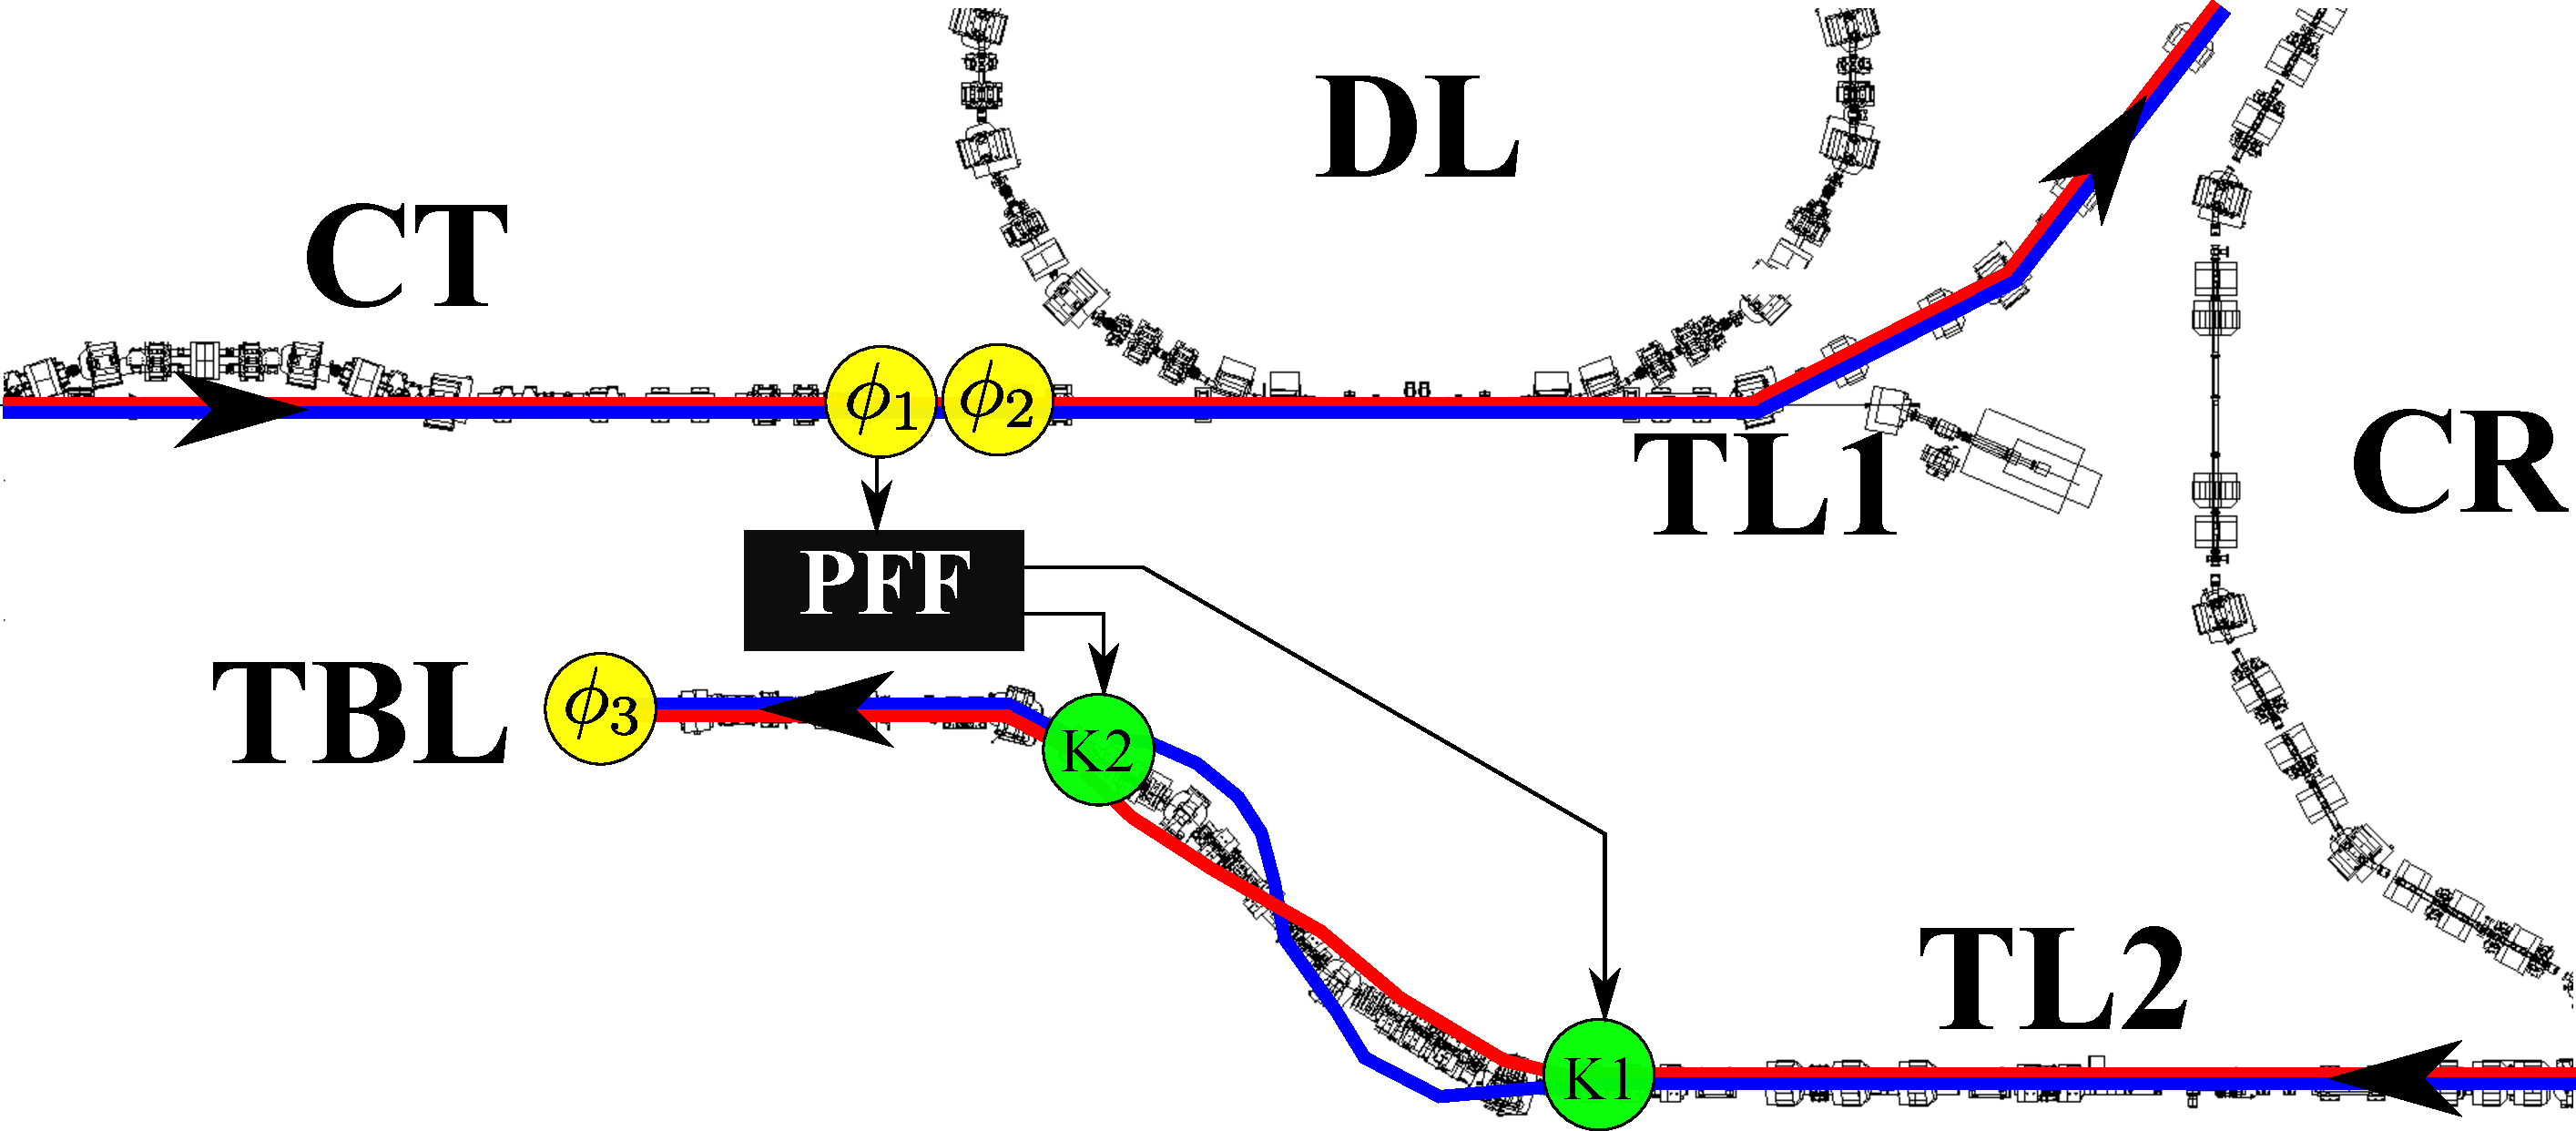
\includegraphics[width=0.5\textwidth]{figs/ctfpffLayout}% Here is how to import EPS art
\caption{\label{fig:pffLayout}Schematic of the PFF system at CTF3.}
\end{figure}

\section{\label{s:ctfLayout}System Design}

The PFF system uses three phase monitors, a digitiser/feedforward controller and two electromagnetic kickers...

Bunches arriving early at the first phase monitor are deflected on to longer trajectories in the chicane, bunches arriving late on to shorter trajectories...

\subsection{\label{ss:hardware}Hardware}

Three phase monitor designed and built by INFN Frascati, and electronics by CERN. Resonant cavities. Signal vertical pair of feedthroughs summed in hybrid. Sum signal mixed with 12~GHz reference. Eight mixers used to achieve both good linearity and resolution. Best measured resolution is 0.126 degrees sampled at 192~MHz...

Two electromagnetic kickers designed and built by INFN Frascati, based on DAFNE design. Horizontal deflection of 1~mrad for voltage of 1.26~kV applied to downstream end of each kicker strip (135~MeV beam)... 

Amplifier designed and built by John Adams Institue/Oxford University. For an input voltage of 2~V gives an output of up to 700~V. Response linear within 3\% for input voltages up to \(1.2\)~V, then starts to saturate. Bandwidth 47~MHz for small signal variations up to 20\% max output...

Feedforward digitiser and controller (FONT5a board) designed and built by John Adams Institute/Oxford University. 9 ADCs, FPGA, 4 DACs... Digitises output from phase monitor electronics, calculates amplifier output based on set gain values, deals with correction timing...

\subsection{\label{ss:hardware}Optics}

Two kickers are placed before first and last dipole in the chicane. Installed inside wide aperture quadrupoles to maintain functionality of the lattice...

Key figure of merit for the PFF optics is the transfer matrix coefficient R52, which relates the applied kick to the resulting phase shift...

PFF system should not degrade transverse stability of beam after chicane. Can be achieved by requiring R11=-1 and R12=0 between kickers...

All this must be achieved whilst keeping dispersion low, matching betas etc. within constraints of pre-existing buildings. Achieved R52 0.74m with max dispersion 1.16m...

But had to accept R56 of -0.18m. Means introduction of additional energy dependent jitter downstream not present upstream. PFF system (at CTF) requires residual R56 below 1cm to achieve 97\% correlation. Created new optics for TL1 line with varying R56, to control this effect...

\subsection{\label{ss:commiss}Commissioning}

(MIGHT BE BETTER TO MERGE POINTS HERE IN TO OTHER SECTIONS?)

Correction range is 5.5 degrees, consistent with kicker design and amplifier output. Means only a portion of the CTF3 pulse can be corrected due to phase sag (or maybe could avoid this by only including central part of pulse in plots)...

Beam time of flight 380~ns between first phase monitor and first kicker. Overall measured system latency is 350~ns, including all hardware and cables. Correct same bunch originally measured...

(Need to) demonstrate that downstream orbit is independent of applied kick...

\begin{figure}
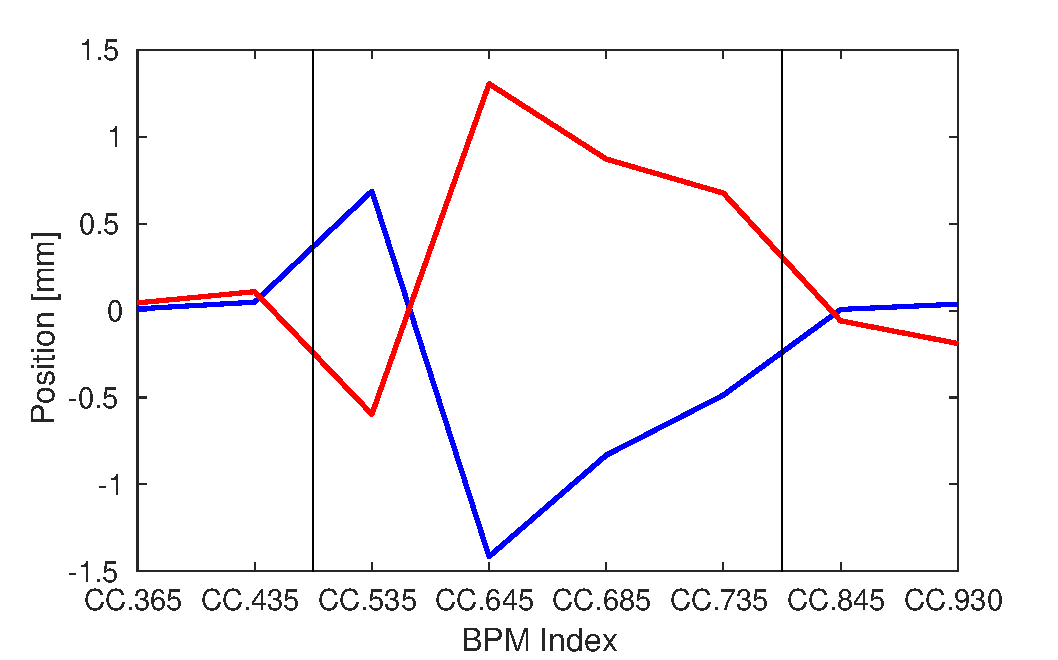
\includegraphics[width=0.5\textwidth]{figs/orbClos}% Here is how to import EPS art
\caption{\label{fig:orbClos}Orbit closure - NEED NEW DATA.}
\end{figure}


\section{\label{s:results}Results}

\subsection{\label{ss:gScan}Gain Scan}

Theoretical limit on the corrected jitter is \(\sigma_d \sqrt{1-\rho_{ud}^2}\)...

Optimal gain value is \(g = \rho \sigma_d/\sigma_u\)...

Would like new data here but would be nice to: have a scan with clear jitter vs. gain relationship (difficult because of propagation drifts). Otherwise, scatter plot like one I've included could be used to demonstrate effect...

\begin{figure}
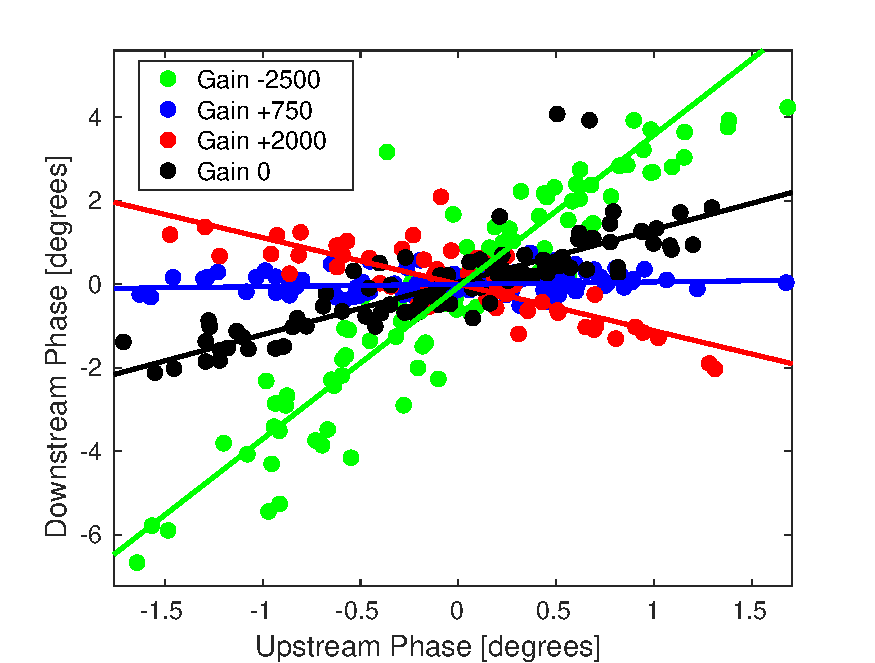
\includegraphics[width=0.5\textwidth]{figs/gScan}% Here is how to import EPS art
\caption{\label{fig:gScan}Gain scan - NEED NEW DATA.}
\end{figure}


\subsection{\label{ss:meanJit}Mean Jitter}

(General question: With/without wiggling, mean and point-by-point -- probably can't include all 4? Which to focus on? Need to at least quote lowest achieved jitter, but wiggling results can look more impressive in plots)

Achieved jitter on the mean phase of 0.24 degrees...

Consistent with theoretical value of (TO CALCULATE) given initial correlation, jitter in this dataset...

Assuming 0.1 degrees resolution on mean (best achieved), measured jitter corresponds to actual beam jitter of 0.22 degrees...

\begin{figure}
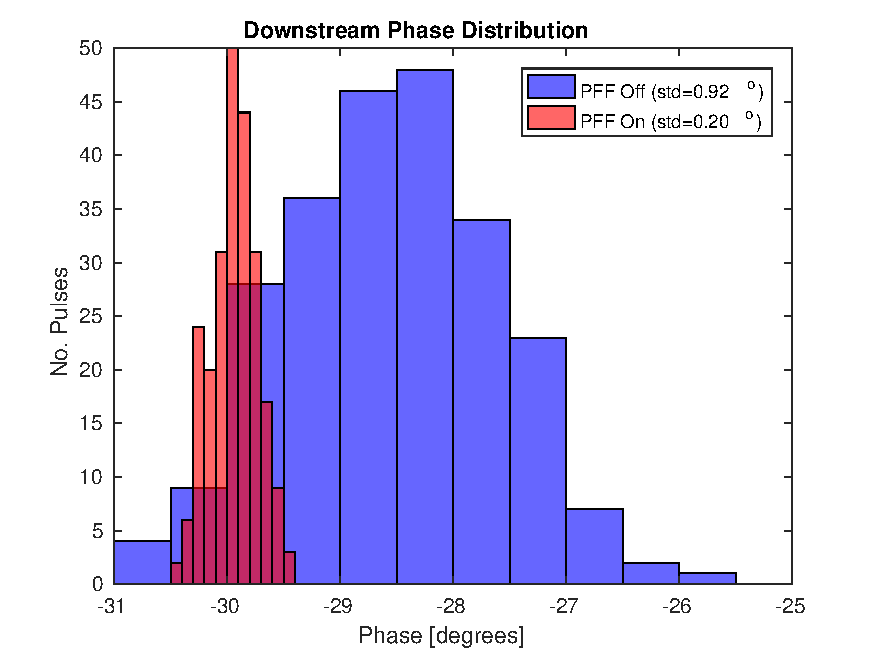
\includegraphics[width=0.5\textwidth]{figs/BestFF_meanJit}% Here is how to import EPS art
\caption{\label{fig:meanJit}Best mean phase jitter.}
\end{figure}


\subsection{\label{ss:shape}Pulse Shape}

High bandwidth correction - not only correcting the mean but also variations along the pulse...

Peak-to-peak variation of 5.76 degrees in initial phase reduced to 0.65 degrees in corrected phase -- OR -- standard deviation of phases reduced from 1.68 to 0.26 degrees...

\begin{figure}
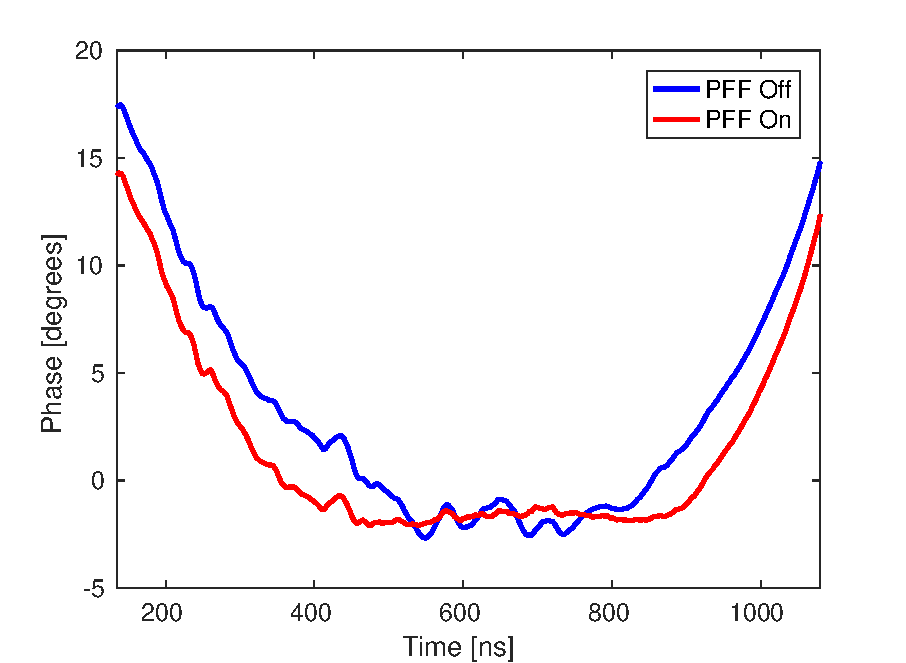
\includegraphics[width=0.5\textwidth]{figs/BestFF_shape}% Here is how to import EPS art
\caption{\label{fig:shape}Correction of pulse shape.}
\end{figure}

\subsection{\label{ss:pbpJit}Point-by-point Jitter}

Point-by-point jitter of x~degrees achieved across a x~ns portion of the pulse, agrees with simulated value...

Limited by variations in phase propagation along the pulse (energy differences etc.), plus resolution slightly worse for point by point than for mean.

\begin{figure}
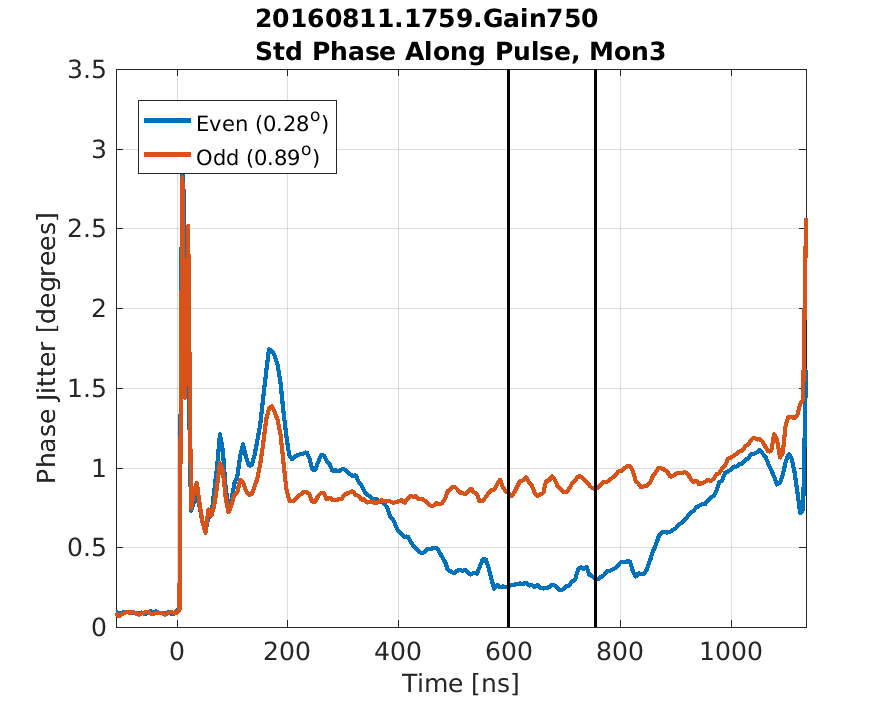
\includegraphics[width=0.5\textwidth]{figs/BestFF_pbp}% Here is how to import EPS art
\caption{\label{fig:BestFF_pbp}Point-by-point jitter.}
\end{figure}


\section{\label{s:conc}Conclusions}

PFF prototype at CTF3 has demonstrated phase stability close to CLIC requirements...

\bibliography{apssamp}% Produces the bibliography via BibTeX.

\end{document}
%
% ****** End of file apssamp.tex ******
